\section{Power}
\label{sec:Power}
The objective of the power system is to provide real-time adjustment of fluid energy input to the manipulators.

%The power system is used in conjunction with the curvature controllers developed in Section~\ref{sec:Control} and the kinematic algorithms developed in Section~\ref{sec:Kinematic Modeling} to achieve closed-loop configuration control of the manipulators.

In general, fluid power can be achieved by controlling either pressure or volume.
We choose volume control because it offers the ability to: (i) measure the control variable via linear displacement as opposed to pressure transducers, (ii) set a maximum safe displacement limit, and (iii) vary pre-pressurization of segments to accommodate for differences in actuator compliance.

\subsection{Fluidic Drive Cylinder}
\label{subsec:Power, FDC}
In order to independently and bidirectionally actuate arm segments, an array of custom fluidic drive cylinders were developed.
These cylinders provide fluidic power to the arm by producing volumetric changes within a segment's embedded channels.
Linear actuators are directly coupled to and control the positional displacements of the pistons within fluidic cylinders.
Accordingly, these linear actuators govern the volumetric displacement of fluid out of the cylinders and into a segment's embedded channels, and vice versa.
Figure~\ref{fig:DriveCylinderOverview} illustrates the components of a fluidic drive cylinder.
\begin{figure}[thb]
\centering
   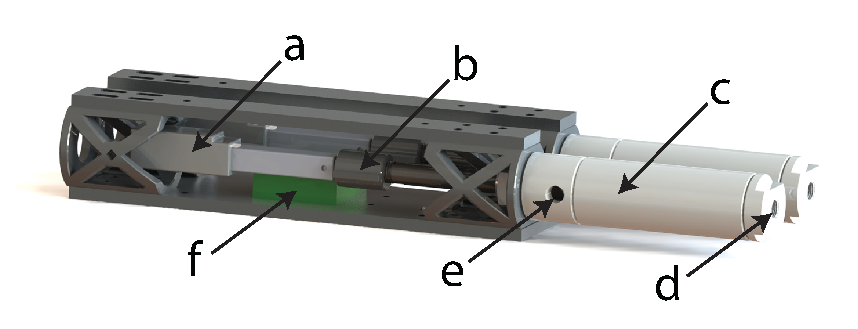
\includegraphics[width=\columnwidth]{Figures/power/DriveCylinderOverview.eps}
   \caption[An overview of the fluidic drive cylinders.]{An overview of two fluidic drive cylinders used to drive the curvature of a bi-directional arm segment. (a) An electric linear actuator$^5$ is directly attached to the piston of a fluidic cylinder$^6$ (c) via a 3D-printed coupler (b). Fluid is displaced through the inlet (e) and outlet (d) of the cylinder. A motor controller$^7$ (f) allows digital command signals to govern fluid movement.}
   \label{fig:DriveCylinderOverview}
\end{figure}

\subsection{Fluidic Drive Cylinder Model}
\label{subsec:Power, Model}
In the following, a model of the fluidic drive cylinder is developed.
Although this plant model is not used in the control of the cylinder, it serves to identify the impact design decisions have on the system's input-output relationships.
Figure~\ref{fig:CylinderModel} shows a simplified schematic representation of the closed-loop fluidic power delivery system.
A linear time-invariant dynamic model can be created to \emph{approximate} the behavior of a fluidic drive cylinder connect to an elastomer channel, and we refer to this as the plant in Figure~\ref{fig:CylinderModel}.

In order to develop the plant model, we make the following assumptions:
\begin{enumerate}
  \item The motor has no inductance. We justify this by observing that the dynamics of the electrical system are considerably faster than the dynamics of the fluidic system.
  \item The piston moves without friction inside the cylinder. We justify this by observing that most of the plant's energy is removed via the highly resistive fluid transmission line between the cylinder and channel.
  \item The channel's compliance $C_c$, which is the ratio of its change in volume to change in pressure, is piecewise constant with respect to channel pressure.
  \item The fluid's compliance $C_f$, which is also the ratio of its change in volume to change in pressure, is constant with respect to fluid pressure. This is, because linearizing the ideal gas law around the operating point $p_0$ at constant temperature $T_0$ leads to $\mathbb{V} = -\frac{m R T_0}{p_0^2} \, p = C_f \, p$.
  \item The fluid's mass is negligible, because we are currently only working with gases, specifically air.
\end{enumerate}

\begin{figure}[htb]
\centering
   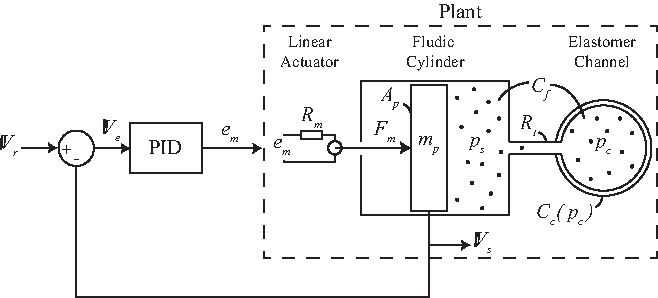
\includegraphics[width=\columnwidth]{Figures/power/CylinderModel}
   \caption[Parameters used in developing a simplified fluidic drive cylinder model.]{Parameters used in developing a simplified fluidic drive cylinder model. A schematic representation of the plant shows a linear electric actuator (left), a piston and fluidic cylinder (middle), and an elastomeric channel grouping within an arm segment (right). A PID controller runs the plant with the volumetric displacement as its reference value, the motor voltage as its control effort and the sensed volumetric displacement as its feedback.}
   \label{fig:CylinderModel}
\end{figure}

The equations of motion for the drive cylinder are expressed in the following. First, the piston's linear motion can be approximated as
\begin{equation}\label{eq:eom1}
    F_m - p_s \, A_p \approx \frac{m_p}{A_p} \ddot{\mathbb{V}}_s,
\end{equation}
where $F_m$ is the force exerted by the linear motor on the piston, $p_s$ is the gauge pressure of the fluid inside the cylinder, $A_p$ is the cross sectional area of the piston, $m_p$ is the mass of the piston, and $\mathbb{V}_s$ is the volumetric displacement of the cylinder.
We can derive the next equation of motion by observing that the total volume of fluid within the plant (represented as the dotted area in Fig.~\ref{fig:CylinderModel}), does not change as this is a closed-circuit drive system.
It follows that $\Delta \, \mathbb{V} \approx 0$ and therefore
\begin{equation}\label{eq:eom2}
    \dot{\mathbb{V}}_s + \dot{p}_s \, C_f + \dot{p}_c \, \left( C_f + C_c \right) \approx 0.
\end{equation}
Here, $p_c$ is the gauge pressure of the fluid within the elastomer channel and $C_f$ and $C_c$ are the compliances of the transmission fluid and elastomer channel, respectively. The volumetric fluid flow into the cylinder is approximated as
\begin{equation}\label{eq:eom3}
    \dot{\mathbb{V}}_s + \frac{p_c - p_s}{R_t} \approx -C_f \dot{p}_s,
\end{equation}
where $R_t$ is the resistance of the fluid transmission line connecting the cylinder and channel. Lastly, the force output of the linear actuator can be approximated as
\begin{equation}\label{eq:eom4}
    F_m \approx - \frac{\beta \, \lambda}{R_m \, A_p} \, \dot{\mathbb{V}}_s + \frac{\beta}{R_m} \, e_m.
\end{equation}
Above, $\beta$ is the motor constant relating motor current to the force of the linear actuator. The motor constant $\lambda$ relates linear velocity to the counter EMF voltage, $R_m$ is the motor's resistance, and $e_m$ is the input motor voltage.

Using these equations of motion, a SISO LTI open-loop plant model can be expressed in the form
$\dot{\mathbf{x}} = \mathbf{A}_{\text{OL}}\,\mathbf{x} + \mathbf{B}_{\text{OL}}\, u$ and
$y = \mathbf{C}_{\text{OL}}\,\mathbf{x}$,
and is explicitly written in Equation~\ref{eq:LTI}.
Combining Equation~\ref{eq:eom1} and \ref{eq:eom4} yields the first row.
The second row is found by combining Equation~\ref{eq:eom2} and \ref{eq:eom3}, and the third row is Equation~\ref{eq:eom3}.

\footnotesize
\begin{align}\label{eq:LTI}
\nonumber  \begin{bmatrix}
  \ddot{\mathbb{V}}_s \\
  \dot{p}_c \\
  \dot{p}_s
  \end{bmatrix} &=
  \setlength{\arraycolsep}{2pt}
  \begin{bmatrix}
  -\frac{\beta \lambda}{m_p R_m} & 0 & -\frac{A_p^2}{m_p} \\
  0 & \frac{1}{\left( C_f + C_c \right) R_t} & -\frac{1}{\left( C_f + C_c \right) R_t} \\
  -\frac{1}{C_f} & -\frac{1}{C_f R_t} & \frac{1}{C_f R_t}
  \end{bmatrix}
  \begin{bmatrix}
  \dot{\mathbb{V}}_s \\
  p_c \\
  p_s
  \end{bmatrix} +
  \begin{bmatrix}
  \frac{\beta A_p}{m_p R_m} \\
  0 \\
  0
  \end{bmatrix} e_{m}\\
  y &=
  \begin{bmatrix} 0 & 1 & 0
  \end{bmatrix}
  \begin{bmatrix}
  \dot{\mathbb{V}}_s \\
  p_c \\
  p_s
  \end{bmatrix}
\end{align}
\normalsize

For bounded-input, bounded-output stability, it is sufficient to use a proportional control law taking the form
\begin{equation}
    e_m(t) = K_p \, \left( \mathbb{V}_r(t) - \mathbb{V}_s(t) \right),
\end{equation}
where $\mathbb{V}_r$ is a reference volume and $K_p$ is a proportional gain constant. However, to ensure zero steady-state error in tracking the reference volume and for a suitable dynamic response, we implement a traditional PID control law
\begin{eqnarray}
    e_m(t) = K_p \,\mathbb{V}_{e}(t) + K_i \, \int_0^t \mathbb{V}_{e}(\tau) \text{d}\tau + K_d \, \frac{\text{d} \mathbb{V}_{e}(t)}{\text{d} t}\\
    \mathbb{V}_{e}(t) = \mathbb{V}_r(t) - \mathbb{V}_s(t).
\end{eqnarray}

Approximations of the model's parameters are listed in Table \ref{tab:ModelParameters}. We approximate the transmission line resistance as
\begin{equation}
    R_t \approx \frac{128 \, \mu \, L_t}{\pi \, d_t^4},
\end{equation}
where $\mu$ is the fluid's viscosity, $L_t$ is the transmission line's length, and $d_t$ is the transmission line's inside diameter.
Figure~\ref{fig:compliancePlot} details the experimentally determined pressure-volume relationship of both the transmission fluid and the compliant elastomer channel.
Channel compliance was determined by actuating a fluidic elastomer actuator with an incompressible fluid and measuring the resulting internal pressuring while incrementally increasing channel volume.
The incompressible fluid enables channel compliance to be decoupled from transmission fluid compliance.
By linearizing this experimental data, the fluid compliance $C_f$ and the piecewise defined channel compliance $C_{c1}$ and $C_{c2}$ can be determined. Also the linearization offset $\mathbb{V}_{\text{off}}$ can be found.
To verify the plant model, model predicted transmission line flow $\frac{p_s - p_c}{R_t}$ was compared to experimentally measured flow (Fig.~\ref{fig:flowVerification}).
To obtain flow data, a flow transducer was placed inline with the transmission tubing.
\begin{figure}[htb]
\centering
   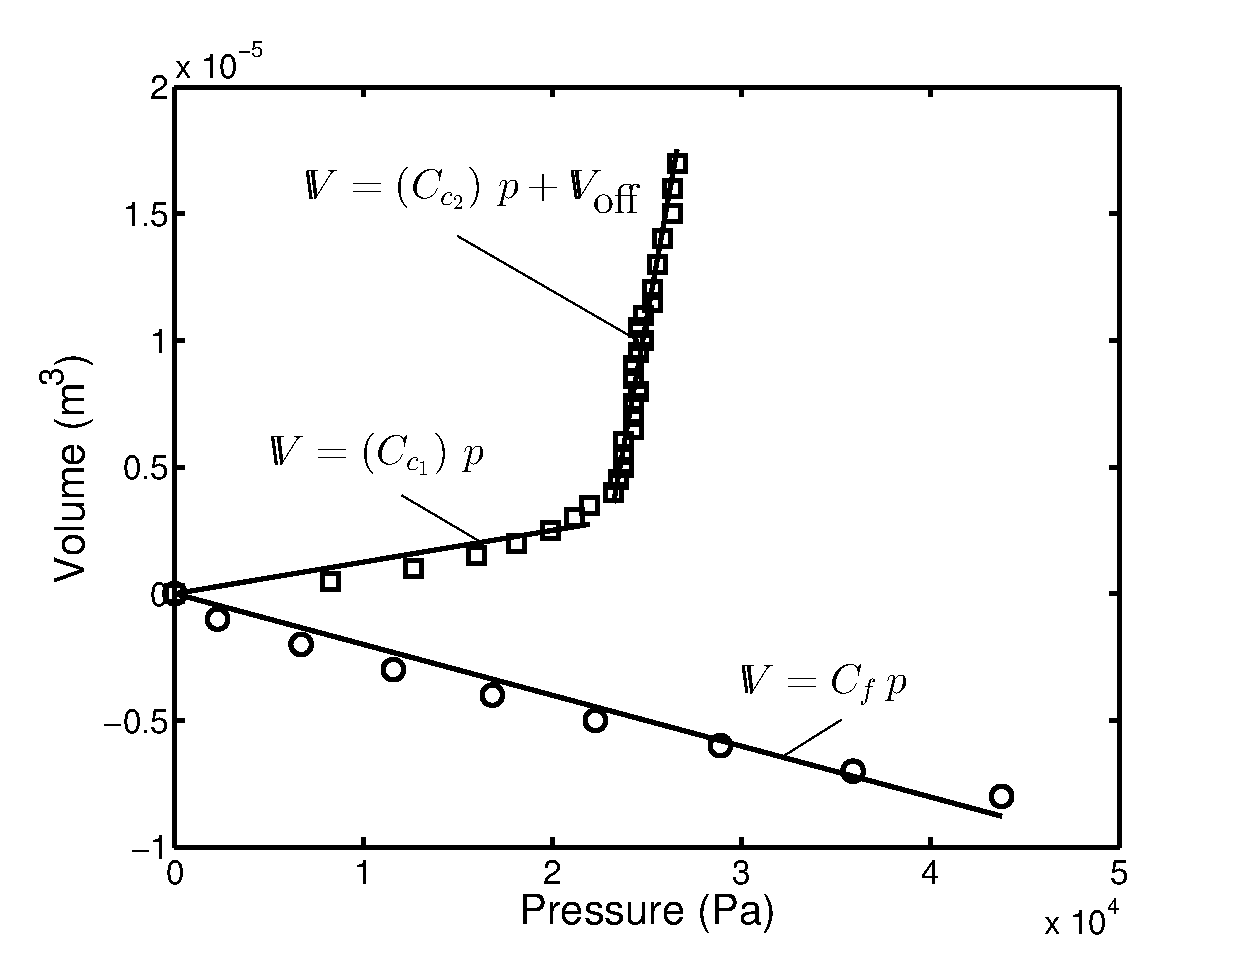
\includegraphics[width=\columnwidth]{Figures/power/compliancePlot_new.eps}
   \caption[Experimentally measured actuator compliance]{Experimentally measured pressure-to-volume relationship of air $(C_f)$ and of air and elastomer channel combined $(C_f + C_c)$.}
   \label{fig:compliancePlot}
\end{figure}

\begin{figure}[htb]
\centering
   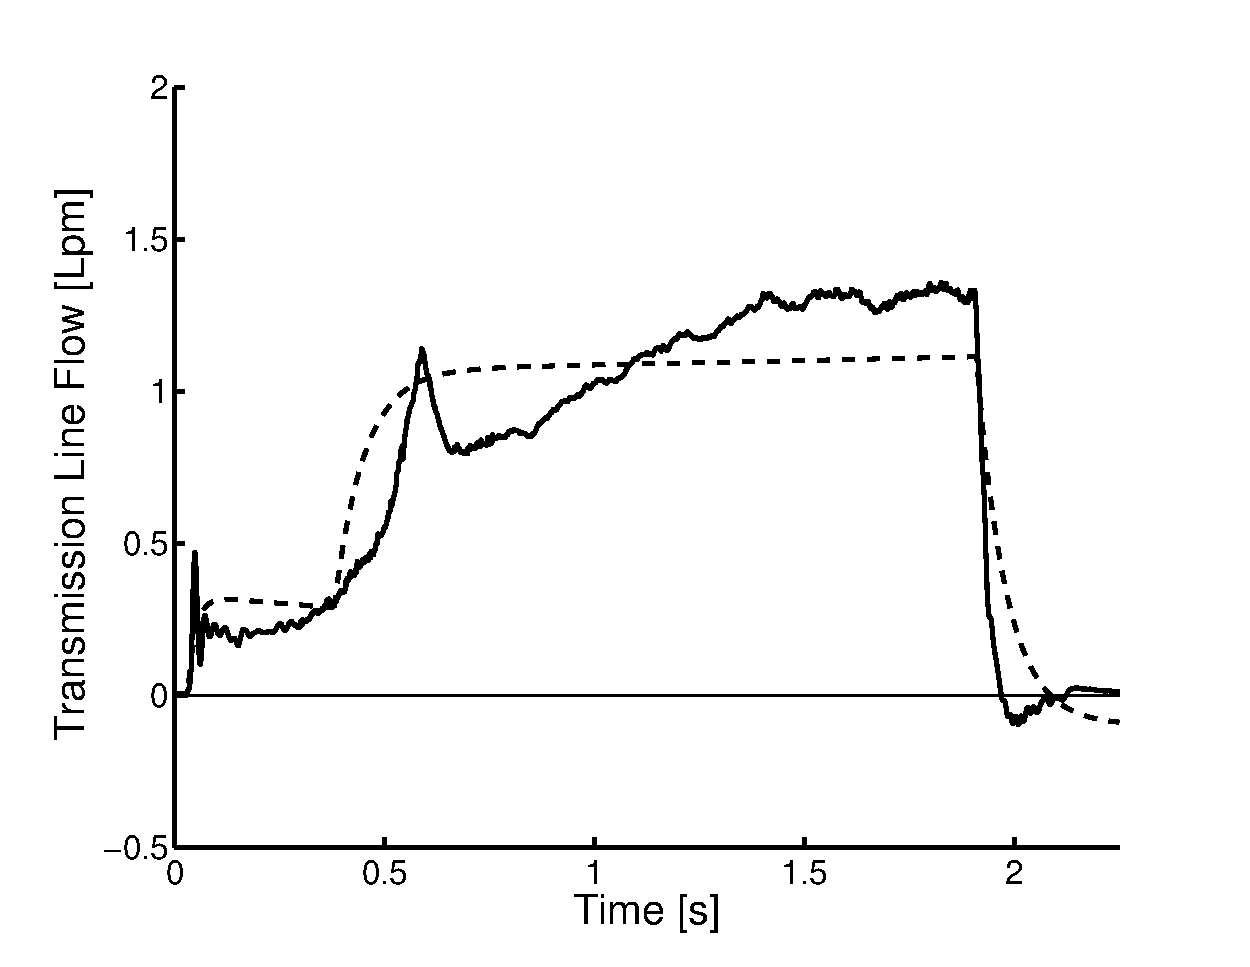
\includegraphics[width=\columnwidth]{Figures/power/flowVerification.eps}
   \caption[Experimental verification of the fluidic drive cylinder plant model.]{Experimental verification of the fluidic drive cylinder plant model. The solid line represents measured transmission line flow, and the dotted line represents model predicted flow.}
   \label{fig:flowVerification}
\end{figure}

\begin{table}[htb]
\centering
\footnotesize
\tabcolsep=0.11cm
\begin{tabular}{c c c c c c c c c c}
\hline\hline
$\beta$ & $\lambda$ & $m_{p}$ & $R_{m}$ & $A_{p}$ & $C_{f}$ & $C_{c1}$ & $C_{c2}$ & $V_{\text{off}}$ & $R_{t}$ \\
232 & 475 & 0.19 & 18.5 & 7.92 & -2.0e-10 & 1.25e-10 & 4.15e-9 & -9.3e-05 & 3.4e8\\
$\frac{\text{N}}{\text{A}}$ & $\frac{\text{V}\text{ s}}{\text{m}}$  & kg & $\Omega$ & \text{cm}$^2$ & $\frac{\text{m}^3}{\text{Pa}}$ & $\frac{\text{m}^3}{\text{Pa}}$ & $\frac{\text{m}^3}{\text{Pa}}$& $\text{m}^3$ & $\frac{\text{Pa s}}{\text{m}^3}$\\[1ex]
\hline
\end{tabular}
\caption{Approximations of fluidic drive cylinder parameters}
\label{tab:ModelParameters}
\end{table}
%C_f = -8.756e-6/4.378e4 = -2.0000e-10
%C_c1 = -8.437e-6/2.661e4 - C_f = 1.1706e-10
%C_c2 = (1.833e-5 - 9.186e-6)/(3.447e4-2.806e4) - C_f = 1.2265e-09
%V_off = 9.186e-6 - (2e-10+1.2265e-9)*2.806e4 = -3.0842e-05

\subsection{Fluidic Drive Cylinder Implementation}
\label{subsec:Power, Implementation}
Fluidic drive cylinders are mechanisms, which interface the computational and algorithmic aspects of the manipulation system with the soft arm.
Specifically, they input digital command signals from a control algorithm and generate fluidic pressure that drives the curvature of the arm segments.

Two drive cylinders are used to control a single bidirectional segment.
Although the mapping of either the agonistic or antagonistic channel deformation is monotonically related to a single piston's displacement, when considering bidirectional segment movement as well as positive and negative curvatures, the two drive cylinders must be controlled synchronously.
One piston is held still and the other piston is moved in either forward or reverse to increase or decrease curvature. There are four distinct states of a pair of fluidic drive cylinders in this arrangement as detailed in Figure~\ref{fig:DriveCylinderStates}.
%First, if the curvature is negative and the error in curvature (red arc - blue arc) is positive, then the cylinder driving the left channel grouping is driven in reverse (top left). Second, if the curvature is positive and the error in curvature is negative, then the right cylinder is driven in reverse (top right). Third, if the curvature is positive and the error positive, the right cylinder is driven forward (bottom left). And lastly, when curvature is negative and the error is negative, the left cylinder is driven forward (bottom right).
\begin{figure}[thb]
\centering
   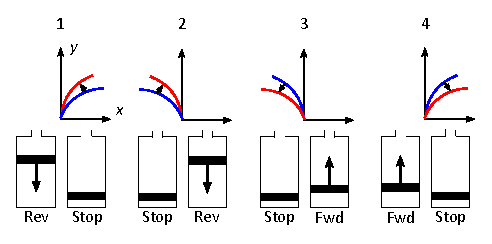
\includegraphics[width=\columnwidth]{Figures/power/DriveCylinderStates.eps}
   \caption[Diagram depicting the driving states of the fluidic drive cylinders]{Diagram depicting the four driving states of the two fluidic drive cylinders used to control an arm segment. These states depend on the error in curvature (measured state shown as blue arcs minus target state shown as red arcs) as well as the sign of the curvature (right hand rule). (\textbf{1}) The curvature is negative and the error is positive. (\textbf{2}) The curvature is positive and the error is negative. (\textbf{3}) The curvature is positive and the error is positive. (\textbf{4}) The curvature is negative and the error is negative.}
   \label{fig:DriveCylinderStates}
\end{figure} 